% source TeXample.net
% modified by Truong Nhan Nguyen

\documentclass[tikz, border=10pt]{standalone}

\usepackage{tikz}
\usetikzlibrary{arrows, shapes, positioning, decorations.markings}

\tikzset{
    arrow style/.style = {scale=1},
    directed/.style = {
        postaction={
            decorate,
            decoration={
                markings,
                mark=at position 0.65 with {\arrow[arrow style]{stealth}}
            }
        }
    },
    reverse directed/.style = {
        postaction={
            decorate,
            decoration={
                markings,
                mark=at position 0.65 with {\arrowreversed[arrow style]{stealth}}
            }
        }
    }
}

\begin{document}
    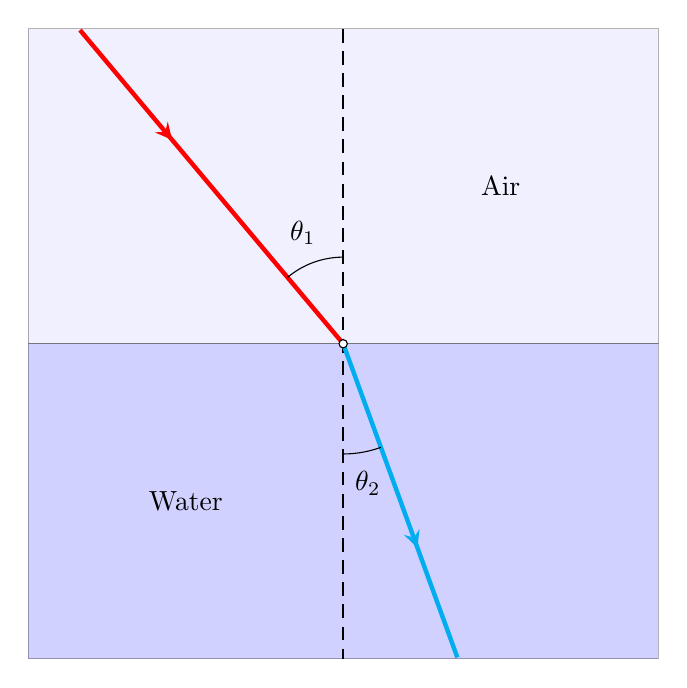
\begin{tikzpicture}
        \coordinate (A) at (0, 4);
        \coordinate (O) at (0, 0);
        \coordinate (B) at (0, -4);
        \coordinate (ml) at (-4, 0);
        \coordinate (ur) at (4, 4);
        \coordinate (lr) at (4, -4);
    
        \draw[fill=blue!20, opacity=.3] (ml) rectangle (ur);
        \draw[fill=blue!60, opacity=.3] (ml) rectangle (lr);
        \draw[dash pattern=on5pt off3pt, thick] (A) -- (B);
        
        \draw (-2, -2) node {Water};
        \draw (2, 2) node {Air};
        
        \draw[red, ultra thick, reverse directed] (O) -- (130:5.2);
        \draw[cyan, ultra thick, directed] (O) -- (-70:4.24);
        \filldraw[fill=white] (O) circle (1.5pt);
        
        \draw (0, 1.1) arc (90:130:1.1);
        \draw (0, -1.4) arc (270:290:1.4);
        \draw (110:1.5) node {$\theta_1$};
        \draw (280:1.8) node {$\theta_2$};
    \end{tikzpicture}
\end{document}